\section{Experimental study}
\label{sec:experiment}

	\subsection{Dataset}
	We implemented our own crawler in Java and started to collect information from YouTube since October, 1st, to November, 5th, 2014. Our crawling strategy is to initialize the crawler with several random "seed" videos, which mostly are in the \textit{Movie} and \textit{Music} category, , and recursively explores all other videos that YouTube suggests as being related to that videos. For each video, we extract all of its metadata such as title, uploader, description, upload date, number of views/likes/dislikes, video length, and a number of other attributes, as well as a list of around 30 videos YouTube recommends as being similar. 

		\subsubsection{Preliminary Data Statistics}

		Although the crawler was suspended twice due to technical issues and upgrades, thus far we have gathered a decent amount of data:

		\begin{itemize}
			\item Number of videos crawled: 1,432,213
			\item Number of uploaders: 628,072
			\item Most viewed video: 2,104,518,656 views.
			\item Most "liked" video: 8,639,650 likes.
			\item Most "disliked" video: 4,184,769 dislikes.
			\item Size of "bag of words" dictionary produced for the titles and descriptions: 2,447,603 entries.
		\end{itemize}

		As the statistics show, we have a large magnitude in ranges of number of view, likes and dislikes. This motivates us to do some preprocessing on data, such as feature normalisation or data standardization, to ensure the numerical stability and good speed of convergence on the learning algorithm. We discuss more on this step in the Section \ref{sec:preprocessing}.
		
		We plot in Figure \ref{fig:logNoOfViews} the distribution of number of views in our current data. Interestingly, the distribution is in the shape of Gaussians, instead of following the Power Law distribution as frequently observed in social network. We guess this observation is due to the way we sample the data, by following the recommended links, and imply that popularity of a video is one of the highly-impacted factors in YouTube recommender systems. Whether we can uncover the underlying reasons of links suggested by YouTube, namely, based on similarity or popularity or both, is an interesting question and may be addressed in our future work.
		
		\begin{figure}[!h]
			\begin{center}
				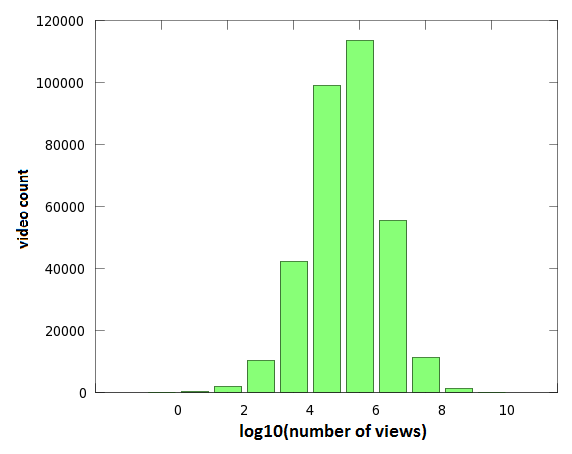
\includegraphics[width=.75\textwidth,clip]{DistributionOfViews.png}				
			\end{center}
			\caption{Histogram on the distribution of number of views (in log-scale).}
			\label{fig:logNoOfViews}
		\end{figure}
				
		\subsubsection{Pre-processing data}
		\label{sec:preprocessing}
		To Joseph: can you help me to work on this part ? You can revise from your discussion of taking the log-form and put it here.
		
		\subsubsection{Feature extraction}
		The first step is to build a dictionary mapping the uploader to the number of videos they have uploaded and the total number of views there videos have. We also take care to prevent "cheating":  In order to ensure that our predictor has only such information as would be available before the video's publishing is ever used, we temporarily reduce these number of video-views and the total number of video uploads for the uploader according to the publish date of the video under current consideration.

	We train a linear regression model for each of our three outputs on the following features:
	\begin{itemize}
		\item
		Many features extracted via a bag-of-words model on the title, using TF-IDF.
	
		\item
		The \# of videos uploaded by the uploader prior to the current video's upload date.

		\item
		The total \# of views for an uploader due to videos released prior to the current video's upload date.
		
		\item
		The fraction of the previous two features (the average number of views per video for videos uploaded by the same uploader prior to the current video's upload date).
		
		\item
		The runtime of the video, in seconds.
	
		\item
		The age of the video at the time of crawling, in days.
	\end{itemize}
	
	\subsection{Evaluation Metrics}
	Three evaluation measures widely used to evaluate ranking approaches are 0-1 loss function, Area under Curve (AUC). \textbf{0-1 loss function} is the ratio of correctly ordered video pairs over total number of pairs in testing set.
	\begin{equation}
		0/1_{loss} = \sum_{(u, v)_{test}} \frac{1}{|(u,v)_{test}|} \textbf{1}[\hat{Y}_{uv} - Y_{uv} == 0]
	\end{equation}
	Since our label values in \{0, 1\}, we use  \textbf{AUC Loss} as another ranking-based performance metric.
	\begin{equation}
		AUC_{loss} = 1 - AUC,
	\end{equation}
	where AUC is the area under the ROC curve.
%\subsection{Comparing Order-of-Magnitude}

%It is important to decide what we will consider as being "close to correct".  0-1 loss is sufficient for our comparison-based version, and for our predictors of the percentage of likes and dislikes, we can simply consider our loss in terms of the square of the difference between our prediction and the true value.  When predicting the number of views, however, we must deal with the gigantic variance in our observed data.

%Ideally, we wish to consider orders of magnitude rather than direct counts, and for this we will set our loss function equal to the square of the difference between the log of our prediction and the log of the observed value.  The motivation is that we wish to reflect the human intuition that there is more difference between the popularities of two videos with 10 and 1,000 views (respectively) than between two videos with 1,000,000 and 1,001,000.  This will prevent petty among between the most popular videos from drowning out the differences in all others.

%The decision to use a log-number-of-views-based loss function may be reversed at a later time if we find better results without it.

%Currently we are using a linear regression to predict the number of views, and we deal with the number of views in log scale for the regression.  One anticipated effect of this is that features will be expected to contribute multiplicitively, rather than additively, to the popularity of a video.  While this certainly seems interesting, it is something that we may ultimately change our minds about as we hone our results to finer detail.  As our model grows more sophisticated than mere linear regression, it may be possible to achieve multiplicitive effects when needed even while working directly with the number of views rather than its log.

	\subsection{Preliminary Results}
	Here we show some of our preliminary results using a simple linear regression.
	
